\chapter{Diseño e implementación} % Main chapter title
En este capítulo se exponen las tomas decisiones referidas al diseño e implementación relacionada al hardware y firmware a lo largo del desarrollo del trabajo. 
\label{Chapter3} % Change X to a consecutive number; for referencing this chapter elsewhere, use \ref{ChapterX}

\definecolor{mygreen}{rgb}{0,0.6,0}
\definecolor{mygray}{rgb}{0.5,0.5,0.5}
\definecolor{mymauve}{rgb}{0.58,0,0.82}

%%%%%%%%%%%%%%%%%%%%%%%%%%%%%%%%%%%%%%%%%%%%%%%%%%%%%%%%%%%%%%%%%%%%%%%%%%%%%
% parámetros para configurar el formato del código en los entornos lstlisting
%%%%%%%%%%%%%%%%%%%%%%%%%%%%%%%%%%%%%%%%%%%%%%%%%%%%%%%%%%%%%%%%%%%%%%%%%%%%%
\lstset{ %
  backgroundcolor=\color{white},   % choose the background color; you must add \usepackage{color} or \usepackage{xcolor}
  basicstyle=\footnotesize,        % the size of the fonts that are used for the code
  breakatwhitespace=false,         % sets if automatic breaks should only happen at whitespace
  breaklines=true,                 % sets automatic line breaking
  captionpos=b,                    % sets the caption-position to bottom
  commentstyle=\color{mygreen},    % comment style
  deletekeywords={...},            % if you want to delete keywords from the given language
  %escapeinside={\%*}{*)},          % if you want to add LaTeX within your code
  %extendedchars=true,              % lets you use non-ASCII characters; for 8-bits encodings only, does not work with UTF-8
  %frame=single,	                % adds a frame around the code
  keepspaces=true,                 % keeps spaces in text, useful for keeping indentation of code (possibly needs columns=flexible)
  keywordstyle=\color{blue},       % keyword style
  language=[ANSI]C,                % the language of the code
  %otherkeywords={*,...},           % if you want to add more keywords to the set
  numbers=left,                    % where to put the line-numbers; possible values are (none, left, right)
  numbersep=5pt,                   % how far the line-numbers are from the code
  numberstyle=\tiny\color{mygray}, % the style that is used for the line-numbers
  rulecolor=\color{black},         % if not set, the frame-color may be changed on line-breaks within not-black text (e.g. comments (green here))
  showspaces=false,                % show spaces everywhere adding particular underscores; it overrides 'showstringspaces'
  showstringspaces=false,          % underline spaces within strings only
  showtabs=false,                  % show tabs within strings adding particular underscores
  stepnumber=1,                    % the step between two line-numbers. If it's 1, each line will be numbered
  stringstyle=\color{mymauve},     % string literal style
  tabsize=2,	                   % sets default tabsize to 2 spaces
  title=\lstname,                  % show the filename of files included with \lstinputlisting; also try caption instead of title
  morecomment=[s]{/*}{*/}
}


%----------------------------------------------------------------------------------------
%	SECTION 1
%----------------------------------------------------------------------------------------
\section{Hardware}
\subsection{Construcción de la válvula de control}
\label{subsec:Construcción de la válvula de control}

En la elaboración del prototipo se creó una caja desmultiplicadora de fuerza con la finalidad de dirigir el recorrido de apertura y cierre de una válvula. Para la generación de estos movimientos se utilizó un servomotor paso a paso.

La válvula es un ensamblaje compuesto de un cuerpo con conexión a una tubería y de un obturador operado por accionamiento. Su función principal es variar el caudal del fluido que circula a través de ella, comportándose como un orificio cuya área está continuamente variando. 
Generalmente el obturador, conforme se va desplazando, produce un área de pasaje que posee una determinada relación característica entre la fracción de carrera y el caudal correspondiente que se escurre a través de ella. Esta relación recibe el nombre de característica inherente de caudal de válvula.

Particularmente, para este trabajo se utilizó una válvula cuya característica inherente es tipo de apertura rápida. Se trata de una propiedad que produce una variación grande de caudal con una carrera pequeña. Esto posibilita el pasaje de casi la totalidad del caudal nominal con apenas una abertura de 25 \% de la carrera total.
De esta forma, genera una ganancia muy alta a bajas aperturas de carrera y una ganancia muy baja en aperturas por encima de 60 \% de carrera total. 
La figura \ref{fig:grafica caudal vs. apertura de valvula}, muestra la curva típica de una válvula de apertura rápida.
\begin{figure}[h]
\centering
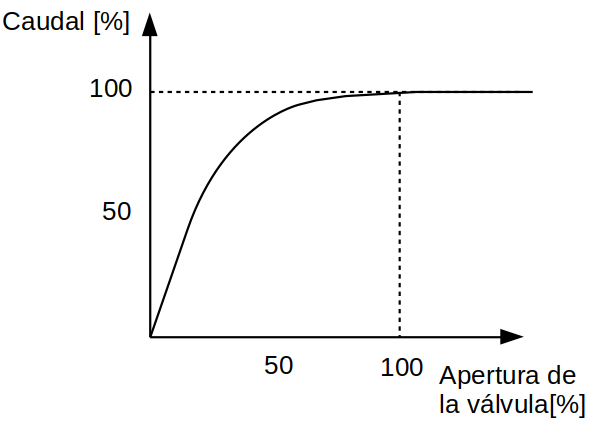
\includegraphics[scale=.60]{./Figures/funcion-valvula.png}
\caption{Gráfica del caudal en función de la apertura de la válvula.}
\label{fig:grafica caudal vs. apertura de valvula}
\end{figure}

\vspace{2cm}
\subsection{Servomotor}
\label{subsec:Servomotor}

Los componentes principales para la construcción del servomotor fueron un motor paso a paso, un controlador, un sensor resistivo de ángulo y una entrada ADC del microcontrolador.


\subsubsection{Circuito interfaz del conector de señal de control P1}

En cuanto a la conexión entre el microcontrolador y el controlador fue necesario la fabricación de un circuito de adaptación de niveles de señales. El MA860H puede aceptar entradas diferenciales y de un solo extremo (incluida la salida de colector abierto y PNP). Tiene 3 entradas lógicas aisladas ópticamente que están ubicadas en el conector P1 para aceptar señales de control del microcontrolador. Estas están aisladas para minimizar o eliminar los ruidos eléctricos acoplados a las señales de control del variador. La figura \ref{fig:circuito interfaz}, ilustra las conexiones a colector abierto.

\begin{figure}[htpb]
\centering
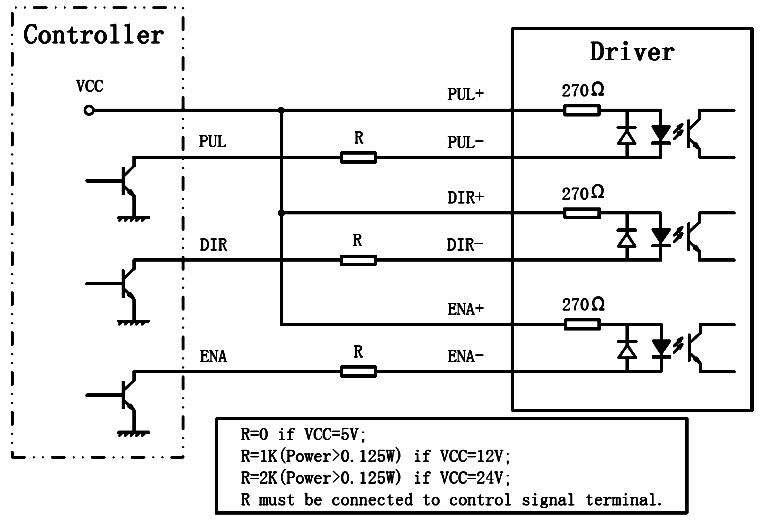
\includegraphics[scale=.55]{./Figures/circuitointerfaz-driver.png}
\caption{Circuito interfaz - conexiones de señales a colector abierto.}
\label{fig:circuito interfaz}
\end{figure}

Siguiendo las recomendaciones del fabricante relacionadas a la construcción del circuito interfaz entre el driver y el microcontrolador se diseñó y fabricó el circuito eléctrico que se muestra en la figura \ref{fig:esquemático circuito interfaz}.

\begin{figure} [htpb]
\centering
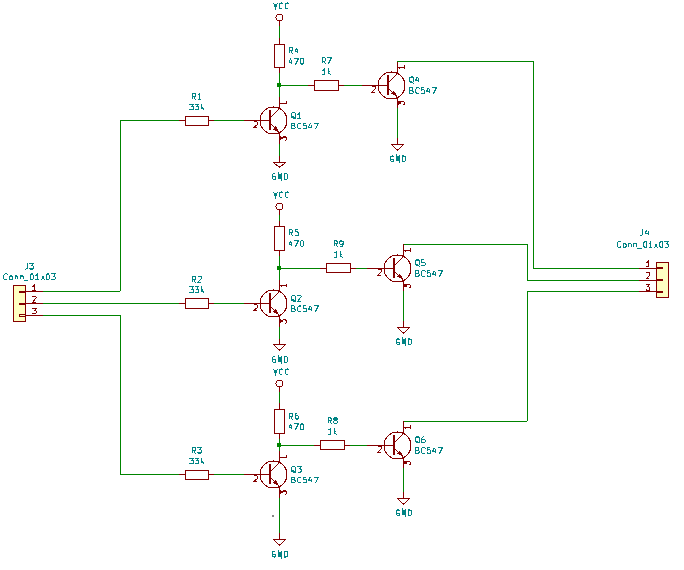
\includegraphics[scale=.85]{./Figures/esquematico-circuito-interfaz.png}
\caption{Esquemático de circuito interfaz entre el microcontrolador y driver.}
\label{fig:esquemático circuito interfaz}
\end{figure}

En el esquemático se observa dos etapas, la primera es un circuito negador y la segunda corresponde a un circuito de colector abierto NPN.
Por lo tanto, se puede decir que la etapa de potencia está formada por el circuito interfaz, el controlador y el motor paso a paso. 

\vspace{3cm}

\subsubsection{Funcionamiento del servomotor}
 
El servomotor está compuesto también por una fracción del firmware que comprende la parte inteligente del dispositivo fabricado.
Asimismo, es el encargado de establecer al obturador de la válvula en una determinada posición y así proporcionar a su salida el caudal de agua requerido por el usuario. 
Para esto fue indispensable obtener una estimación del porcentaje de apertura de la válvula. Por ello, se empleó un sensor resistivo de ángulo cuya señal se inyecta de forma retroalimentada a una de las entradas ADC del microcontrolador para su procesamiento. Este dispositivo adosado al eje de la válvula es un potenciómetro de una vuelta de 50 k$\Omega$ cuyo modelo es 91A-503, Bourns Cermet.

En la figura \ref{fig:Diagrama en bloque de la celda primaria}, se puede apreciar un diagrama en bloque general que indica entre otras partes del trabajo, cómo está constituido el servomotor. Cada componente se encuentra delimitado en líneas punteadas de forma tal, que se puede tener una idea sobre qué partes pertenecen al servomotor y al microcontrolador.   
   

\begin{figure}[htpb]
\centering
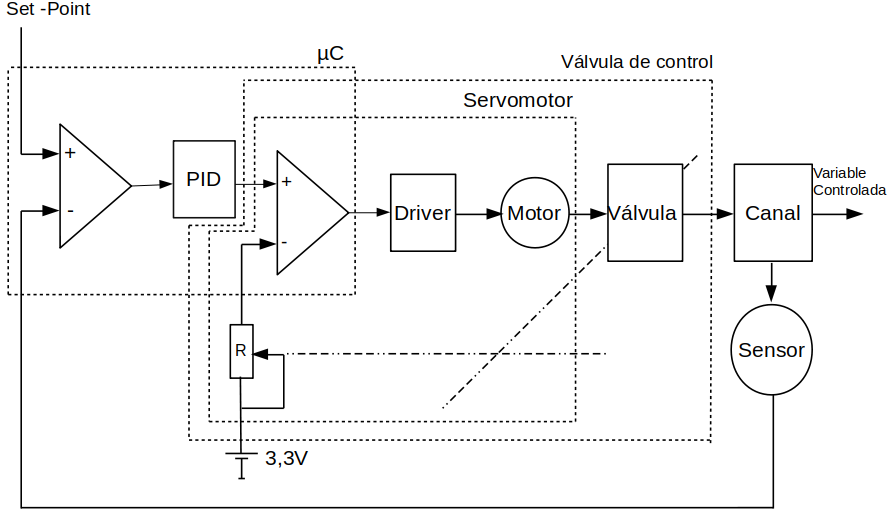
\includegraphics[scale=.65]{./Figures/DiagramaEnBloqueConServoMotor-V2.png}
\caption{Diagrama en bloque de la celda primaria.}
\label{fig:Diagrama en bloque de la celda primaria}
\end{figure}


\subsection{Medidor de caudal}
\label{subsec:Medidor de caudal}
La medición del agua, también llamada aforo, es la cuantificación del caudal de agua que pasa por la sección transversal de un río, canal o tubería. 
En la mayoría de los casos, la medición del agua resulta de la necesidad de brindar mayor control sobre su uso y distribución. Dicha medición se realiza a través de medidores de caudal. Estos son dispositivos que utilizan diferentes principios mecánicos o físicos para permitir que un flujo de agua pueda ser cuantificado. 
La herramienta de medición utilizada en este trabajo para verificar el caudal de agua proporcionado, recibe el nombre de medidor de caudal de canal abierto tipo aforo.

\vspace{1cm}
Existen varias formas de aforo en canales abiertos, dentro de las principales se encuentran:
\begin{enumerate}
	\item Método volumétrico.
	\item Vertederos.
	\item Canal Parshall. 
	\item Método hidráulico.
\end{enumerate}
Para efectuar el presente trabajo se utilizó el tipo de aforo con vertedero triangular con escotadura en V.
La medición del caudal de las corrientes naturales nunca puede ser exacta debido a que el canal suele ser irregular y por lo tanto es irregular la relación entre nivel y caudal. Los canales de corrientes naturales están también sometidos a cambios debidos a erosión o depósitos. Se pueden obtener cálculos más confiables cuando el caudal pasa a través de una sección donde esos problemas se han limitado. Los vertederos pueden ser definidos como simples aberturas, sobre las cuales un líquido fluye. El término se aplica también a obstáculos en el paso de la corriente y a las excedencias de los embalses. Los vertederos son orificios sin el borde superior y ofrecen las siguientes ventajas en la medición del agua: 

\begin{itemize}
\item Se logra con ellos precisión en los aforos 	
\item La construcción de la estructura es sencilla
\item No son obstruidos por materiales que flotan en el agua 
\item La duración del dispositivo es relativamente larga
\end{itemize}
Los vertederos son utilizados, intensiva y satisfactoriamente en la medición del caudal de pequeños cursos de agua y conductos libres, así como en el control del flujo en galerías y canales.
Para la construcción del vertedero triangular empleado, se precisó de una chapa de hierro plana de 1 mm de espesor, a la que se le  realizó una hendidura de sección triangular, cuyo  valor de ángulo es de 18 grados.
Esta chapa supera los límites del ancho del canal de forma que, ubicándola  verticalmente y en forma transversal al canal, opera como un embalse que por su hendidura sale un flujo de agua.
De esta forma se puede medir en distintos lugares del recorrido del canal, cuál es el caudal real que está pasando por ese punto en particular.  
La figura \ref{fig:Placa de aforo},  muestra la vista de frente de una estructura de un vertedero con escotadura en V. 	

\begin{figure}[htpb]
\centering
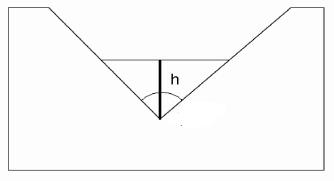
\includegraphics[scale=.75]{./Figures/PlacaDeAforo.jpeg}
\caption{Placa de aforo: vista de frente.}
\label{fig:Placa de aforo}
\end{figure}

\vspace{1cm}
La figura \ref{fig:Placa de aforo-VistaLateral}, ilustra la vista lateral del vertedero y cómo fluye el líquido por su abertura.

\begin{figure}[htpb]
\centering
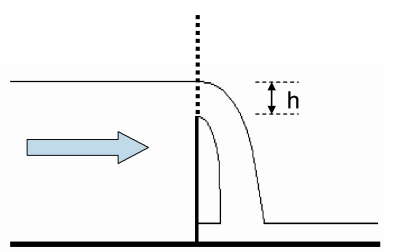
\includegraphics[scale=.75]{./Figures/PlacaDeAforo-VistaLateral.png}
\caption{Placa de aforo: vista lateral.}
\label{fig:Placa de aforo-VistaLateral}
\end{figure}

Entonces, para calcular el caudal se debe tener en cuenta la siguiente fórmula:
\begin{equation}
 \label{eq:caudal}
 Q = \frac{8}{15}\sqrt{2g} c \tan\alpha  H^\frac{2}{5} 
\end{equation}
	
\begin{figure}[htpb]
\centering
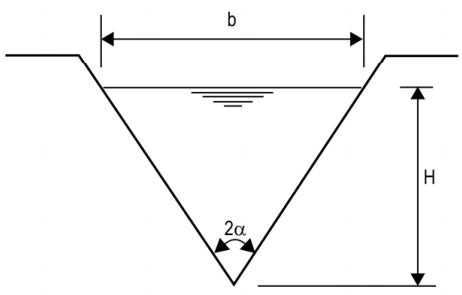
\includegraphics[scale=.75]{./Figures/DimensionesPlacaAforo.png}
\caption{Placa de aforo: dimensiones.}
\label{fig:Placa de aforo dimensiones}
\end{figure}	

Teniendo en cuenta la ecuación \ref{eq:caudal}

\begin{itemize}
\item Q: es caudal en $\frac{m^3}{s} $
\item g: coeficiente de gravedad
\item c: coeficiente de descarga
\item $\alpha$: ángulo del vertedero
\item H: nivel de agua en metros
\end{itemize}

Los medidores de caudal con aforo triangular como el utilizado en el presente trabajo, responden a una ecuación del modelo que se expone arriba obtenida empíricamente.El medidor utilizado en este proyecto se usó por única vez, por lo tanto la tabla de calibración del caudalímetro fue obtenida experimentalmente.  
En la figura \ref{fig:alturas vertedero}, se detalla la vista de frente del canal con el vertedero triangular y los diversos niveles de altura que se consideraron al momento de realizar las mediciones pertinentes. 

\begin{figure}[htpb]
\centering
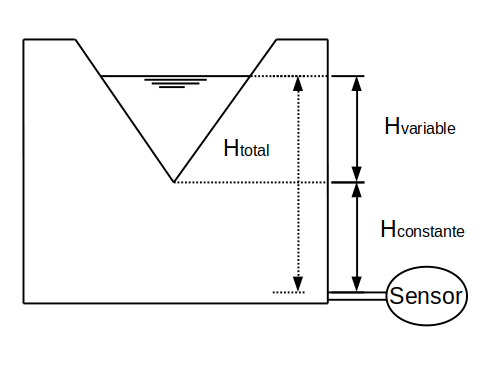
\includegraphics[scale=.75]{./Figures/EsquemaMedicionPresion.png}
\caption{Placa de aforo: dimensiones.}
\label{fig:alturas vertedero}
\end{figure}

A partir de la figura \ref{fig:alturas vertedero} se simboliza una manguera, conectada por un extremo a la base del canal y, en el otro, a una de las dos espigas del sensor. Además, se puede advertir los niveles de altura que se deben tener en cuenta. $H_{total}$ corresponde a la altura entre el nivel de agua en un instante dado y la manguera conectada al sensor, $H_{constante}$ se encuentra asociada al nivel de altura que está comprendido entre dicha manguera y el vértice del triángulo del vertedero, y finalmente $H_{variable}$ es la altura que está contenida entre el nivel de agua y el vértice del triángulo de dicho vertedero.    
Por lo tanto, este caudalímetro de canal abierto por sistema de aforo utiliza como medidor de nivel de columna de agua un sensor de presión cuyo modelo es MPX5010DP. 

Esta señal proveniente del sensor en conjunto con un algoritmo de control PID, permite regular el caudal de agua en un determinado valor preestablecido. 

Una vez construido el prototipo, se realizó una calibración de caudal obteniéndose una tabla de Caudal vs $H_{total}$ (altura). Esta es utilizada en el firmware para obtener el valor de caudal en lugar de la fórmula presentada.

\section{Software}
\subsection{Arquitectura de software}
\label{subsec:Arquitectura de software}

Durante la definición de la arquitectura de software se seleccionaron dos  y se las integraron para confeccionar una híbrida, de modo tal que se adapte a las necesidades concretas de este proyecto. Por un lado, se seleccionó una arquitectura que está conformada por tres capas claramente definidas.
En la capa HAL se encuentran los drivers encargados de abstraer los detalles de acceso al hardware. De esta forma, facilitará la migración a otro microcontrolador en caso de que en el futuro hiciera falta. Adicionalmente, permite una mayor claridad en la implementación, al separar los drivers de la lógica de la aplicación.
Debido a que en la producción se utilizará como hardware a la CIAA-NXP y durante el desarrollo a la EDU-CIAA-NXP, se empleó el firmware de la CIAA versión 3.0 como capa de abstracción de hardware. 
En la capa de aplicación se encuentran todos los componentes que encapsulan la lógica de aplicación, y finalmente, la tercera corresponde al sistema operativo de tiempo real FreeRTOS \citep{FREERTOS}.
El sistema incluye sensores que proveen información relacionada al ámbito a controlar y un actuador para operar sobre el sistema. Por lo tanto, en respuesta a las alteraciones identificadas por los sensores, se envían señales de control a los actuadores. Entonces, al identificar que el sistema debe poseer este tipo de comportamiento se definió emplear una arquitectura de tiempo real inherente al “Control Ambiental” \citep{INGSOF} , ya que este patrón de arquitectura de software brinda la posibilidad de recopilar datos del entorno por medio de sensores como así también el estado en el que se encuentran los actuadores conectados al sistema. Con base en datos reunidos de sensores y actuador, se envían señales de control hacia el actuador para producir cambios en el entorno controlado. En la figura \ref{fig:Arquitectura de software}, se puede ver el diagrama del patrón arquitectónico que es la base del diseño del sistema de control, y además utilizado en la capa aplicación. 

\begin{figure}[htpb]
\centering
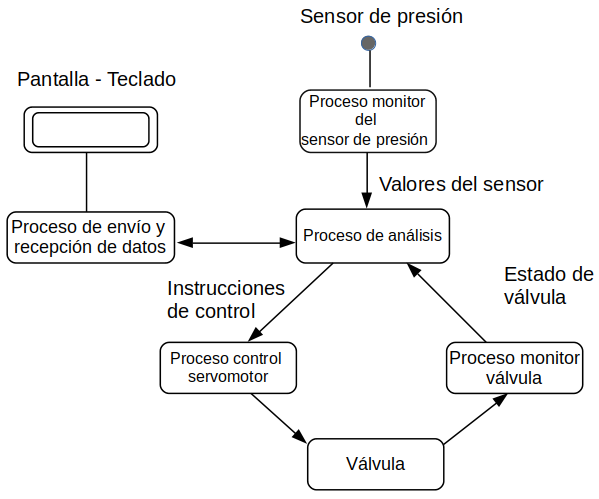
\includegraphics[scale=.65]{./Figures/ArquitecturaSoftware.png}
\caption{Arquitectura de sistema de control de caudal de agua en canal a cielo abierto.}
\label{fig:Arquitectura de software}
\end{figure}

Al aplicar ambos patrones se constituyó un patrón híbrido de tres capas. La capa inferior es la capa de abstracción de hardware. La capa superior, pertenece a la aplicación que incluye los componentes de un patrón control ambiental.

%\vspace{2cm}

\subsection{Componentes de software}
\label{subsec:Componentes de software}
Cada capa de software es considerada un componente de software. Con lo cual se poseen los siguientes componentes:

\begin{itemize}
\item HAL
\item Sistema Operativo
\item Aplicación
\end{itemize}
%\vspace{1cm}
A su vez, la capa de aplicación está compuesta por los siguientes componentes de software:

\begin{itemize}
\item Monitor sensor de presión.
\item Control servomotor.
\item Monitor válvula.
\item Control de recepción y envío de datos.
\end{itemize}

En la figura \ref{fig:Capas de componentes de software}, se puede apreciar el nivel de jerarquía de cada una de las capas donde la capa HAL la  más baja: 

\begin{figure}[htpb]
\centering
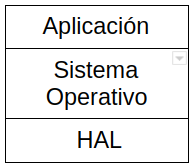
\includegraphics[scale=.65]{./Figures/JerarquiaDeCapas-Software.png}
\caption{Jerarquía de componentes de software.}
\label{fig:Capas de componentes de software}
\end{figure}

\subsubsection{Diseño detallado}
En esta subsección se incluye el diseño detallado de cada uno de los componentes de software presentados en la figura \ref{fig:Arquitectura de software}, todos ellos con sus respectivos diagramas de actividades \citep{DIAGRAMADEACTIVIDADES}. 

	\begin{figure}[htpb]
	\centering
	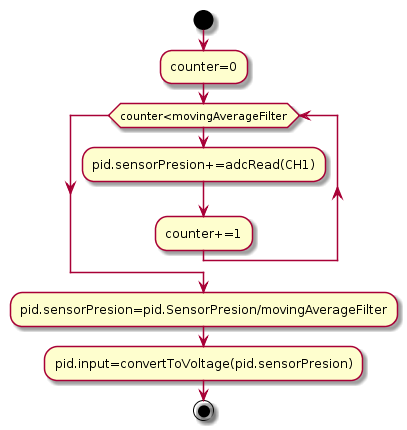
\includegraphics[scale=.65]{./Figures/Procesomonitorsensordepresion.png}
	\caption{Proceso monitor del sensor de presión.}
	\label{fig:Control servomotor}
	\end{figure}
	
\begin{figure}[htpb]
	\centering
	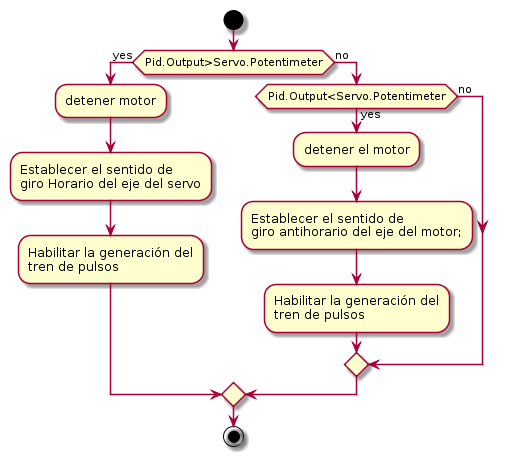
\includegraphics[scale=.65]{./Figures/ProcesoControlServo.png}
	\caption{Proceso de control del servomotor.}
	\label{fig:Control servomotor}
	\end{figure}

 	\begin{figure}[htpb]
	\centering
	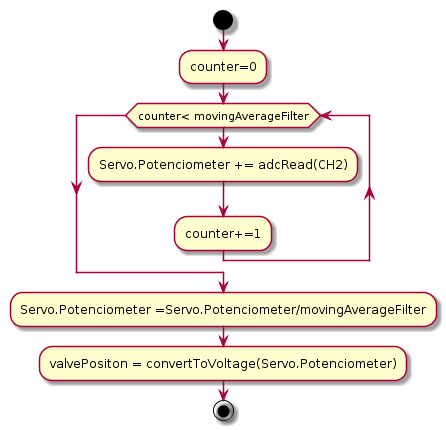
\includegraphics[scale=.65]{./Figures/MonitorValvula.png}
	\caption{Proceso monitor válvula.}
	\label{fig:Proceso monitor valvula}
	\end{figure}

	\begin{figure}[htpb]
	\centering
	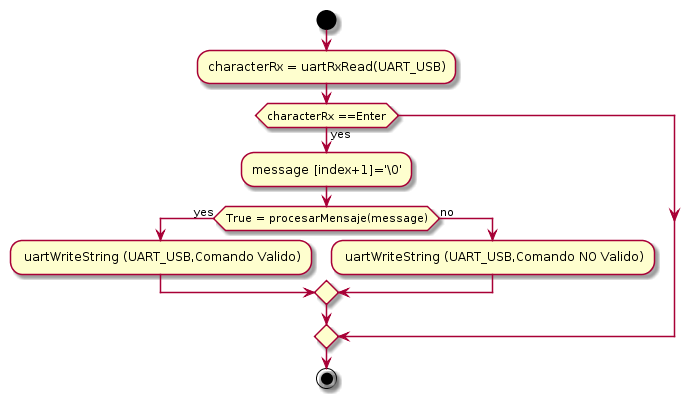
\includegraphics[scale=.65]{./Figures/Porcesorecepcionyenviodedatos.png}
	\caption{Proceso de envío y recepción de datos.}
	\label{fig:Proceso De envió y recepción de datos}
	\end{figure}

	
\begin{figure}[htpb]
	\centering
	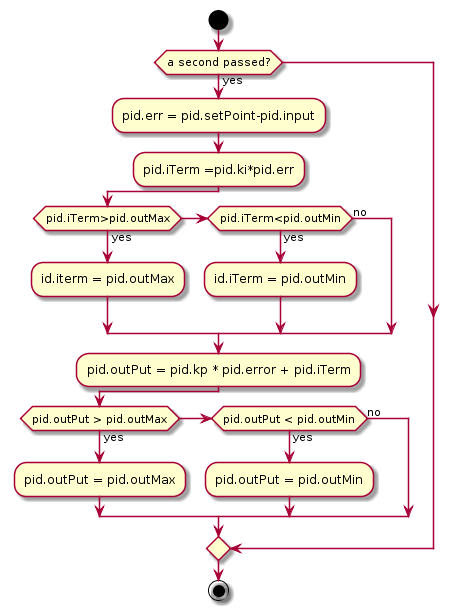
\includegraphics[scale=.60]{./Figures/procesocontrolPID.png}
	\caption{Proceso de control PID.}
	\label{fig:Proceso de Control PID}
	\end{figure}
	
%\vspace{3cm}

\subsection{Casos de uso}
\label{subsec:Casos de uso}
En la etapa de captura de requerimientos funcionales que el sistema debía satisfacer, se emplearon casos de uso correspondientes al Lenguaje Unificado Modelado (UML) \citep{LIBROUML}. Esta técnica es de mucha utilidad y permite especificar, visualizar, construir y documentar los requisitos del sistema especialmente en sistemas con un alto grado de interacción hombre/máquina \citep{PLANTUML}. 
En las tablas \ref{tab:detectar el nivel de agua del canal} y \ref{tab:establecer un determinado valor de caudal.} se presentan dos casos de uso que se documentaron como parte integral de la especificación de requisitos del software del equipo.


\begin{table}[H]
\begin{center}
\caption{ Caso de uso: detectar el nivel de agua del canal.}
\begin{tabular}{ | m{4cm} | m{9.5cm} | }
\hline Nombre & Detectar el nivel de agua del canal \\ \hline
1.1 Breve descripción & 
El firmware debe detectar por medio del sensor de presión el nivel de agua existente en el canal. \\ \hline

 1.2 Actor Principal&La aplicación móvil.\\ \hline


 1.3 Disparadores & La recepción de un comando. \\ \hline

Flujo de Eventos& \\ \hline

 2.1 Flujo básico &
El firmware recibe el comando desde un smartphone  o desde una aplicación de comunicación serial desde una pc. \\ \hline


 2.1.2 Flujo básico &
El firmware deberá desencapsular el comando recibido y extraer los diferentes campos de información. \\ \hline

 2.1.3 Flujo básico &
El firmware deberá identificar el tipo de operación. \\ \hline


 2.1.4 Flujo básico &
El firmware deberá leer un pin configurado como adc asociado al sensor de presión un valor digital. \\ \hline
 

2.1.5 Flujo básico &
Se repite el paso 2.1.4 hasta 5 veces, de forma que el firmware deberá realizar una acumulación de los valores obtenidos. \\ \hline


2.1.6 Flujo básico &
 El firmware con base al acumulador obtenido en el punto anterior deberá, realizar un filtro de promedio móvil.  \\ \hline
 
2.1.7 Flujo básico &
El firmware deberá convertir el valor digital promediado a voltaje. \\ \hline 
2.1.8 Flujo básico &
El firmware deberá obtener el nivel de agua con el dato obtenido en el punto anterior empleando una tabla que se obtendrá experimentalmente. \\ \hline
2.1.9 Flujo básico &
El firmware deberá controlar si el resultado se encuentra dentro de las dimensiones establecidas. \\ \hline
2.1.10 Flujo básico &
El firmware deberá enviar por el puerto serial el valor de nivel de agua en el orden de los centímetros. \\ \hline
2.2 Flujo alternativo &  \\ \hline


2.2.1 Flujo alternativo  & 
2.1.9 Si la distancia obtenida se encuentra fuera de rango se enviará por la UART “Distancia Fuera de Rango - Verificar el correcto Funcionamiento del  sensor”. \\ \hline

Requisitos Especiales & \\ \hline


Pre - condiciones & \\ \hline
 
4.1 Pre - condiciones & 
El firmware debe estar en estado de correcto funcionamiento. \\ \hline

4.2 Pre - condiciones &
La comunicación serial se debe encontrar en condiciones óptimas para su funcionamiento correcto. \\ \hline

Post- Condiciones &
El firmware deberá quedar operativo y en correcto 
funcionamiento y en condiciones para la recepción de futuros comandos. \\ \hline

\end{tabular}

\label{tab:detectar el nivel de agua del canal}
\end{center}
\end{table}

\begin{table}[H]
\begin{center}
\caption{ Caso de uso: establecer un determinado valor de caudal.}
\begin{tabular}{ | m{4cm} | m{9cm} | }
\hline 
Nombre & Establecer un determinado de valor de caudal.\\ \hline
1.1 Breve descripción &
El firmware debe establecer un caudal mediante la manipulación de la posición de la válvula de control.\\ \hline
 1.2 Actor Principal & La aplicación móvil.\\ \hline
 1.3 Disparadores & La recepción de un comando \\ \hline
Flujo de Eventos & \\ \hline


 2.1 Flujo básico &
El firmware recibe el comando desde un smartphone  o desde una aplicación de comunicación serial desde una pc. \\ \hline
 2.1.2 Flujo básico &
El firmware deberá desencapsular el comando recibido y extraer los diferentes campos de información. \\ \hline
 2.1.3 Flujo básico &
El firmware deberá interpretar el tipo de operación. \\ \hline


 2.1.4 Flujo básico &
El firmware deberá leer un pin configurado como adc asociado al sensor de presión un valor digital. \\ \hline


2.1.5 Flujo básico &
Se repite el paso 2.1.4 hasta 5 veces, de forma que el firmware deberá realizar una acumulación de los valores obtenidos.\\ \hline
2.1.6 Flujo básico &
 El firmware con base al acumulador obtenido en el punto anterior deberá, realizar un filtro de promedio móvil.  \\ \hline
2.1.7 Flujo básico & 
El firmware deberá convertir el valor digital promediado a voltaje.  \\ \hline
2.1.8 Flujo básico & 
El firmware deberá obtener el caudal con el dato obtenido en el punto anterior empleando una tabla que se obtendrá experimentalmente. \\ \hline
2.1.9 Flujo básico &
El firmware deberá comparar este resultado de caudal obtenido con el set point. \\ \hline
2.1.10 Flujo básico &
En caso de ser valores diferentes, el firmware deberá generar una señal  tren de pulsos en el sentido correspondiente hasta posicionar la válvula de control. \\ \hline
2.1.11 Flujo básico &
Se repite desde 2.1.4 hasta que el caudal obtenido a través del sensor y el set point sean iguales. \\ \hline
2.2 Flujo alternativo & \\ \hline


2.2.1 Flujo alternativo & 
2.1.10 Si los valores son iguales el firmware deberá detener la generación del tren de pulsos. \\ \hline
Requisitos Especiales & \\ \hline


Pre - condiciones & \\ \hline
 
4.1 Pre - condiciones &
El firmware debe estar en estado de correcto funcionamiento. \\ \hline
4.2 Pre - condiciones &
La comunicación serial se debe encontrar en condiciones óptimas para su funcionamiento correcto. \\ \hline
Post- Condiciones &
El firmware deberá quedar operativo y en correcto funcionamiento y en condiciones para la recepción de futuros comandos.\\ \hline
\end{tabular}

\label{tab:establecer un determinado valor de caudal.}
\end{center}
\end{table}

%\vspace{2cm}


\subsection{Diagrama de clases del firmware}
\label{subsec:Diagrama de clase}
Previo al desarrollo del firmware, se realizó un diagrama de clases \citep{DIAGRAMADECLASES}, que se puede apreciar en la figura \ref{fig:Diagrama de clase.}. 
\begin{figure}[h]
	\centering
	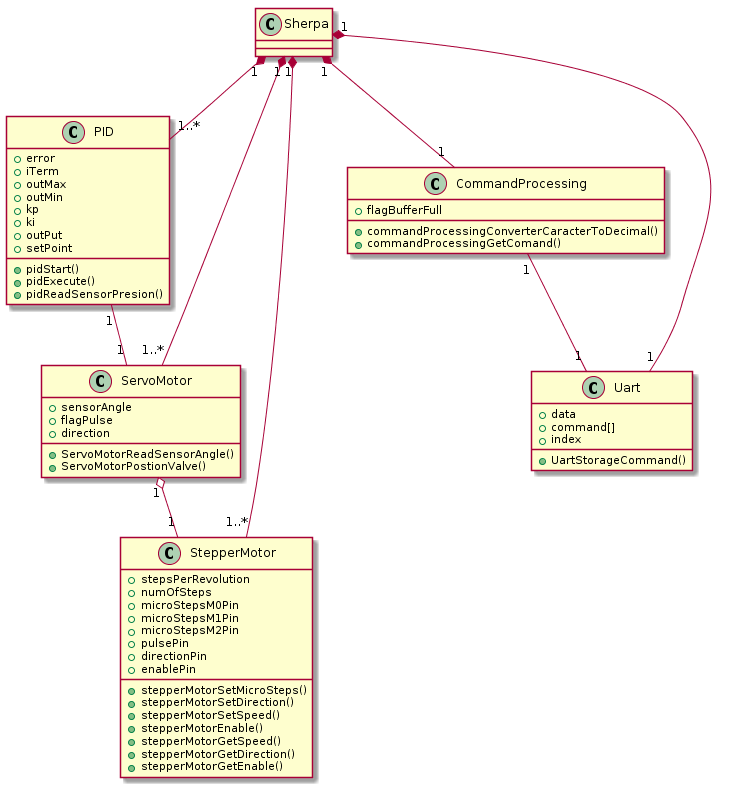
\includegraphics[scale=.50]{./Figures/DiagramaDeClase-DistribucionDeAguaII.png}
	\caption{Diagrama de clases.}
	\label{fig:Diagrama de clase.}
	\end{figure}
\begin{itemize}

\item Uart: este módulo recibe y envía los comandos desde y hacia la aplicación de comunicación serial que se ejecuta en la PC.

\item CommandProcessing: acumula y convierte de carácter a decimal los comandos recibidos y los devuelve cuando es solicitado.

\item StepperMotor: este módulo posee todas las funciones inherentes al control del motor paso a paso. Interactúa con el módulo Servomotor para integrar las características de un servomotor convencional. 

\item ServoMotor: este módulo tiene la misión de establecer en cierta posición al obturador a través de la generación de una señal de tren de pulsos. Esto se realiza mediante una comparación entre la salida del algoritmo de control PID y la señal del sensor resistivo de ángulo. Cuando la comparación resulta igual a cero implica que alcanzó situar el obturador en la posición deseada.

\item PID: este módulo implementa un algoritmo de control PID que se ejecuta cada un segundo para cuantificar el error o desviación que existe entre el valor de caudal medido a través del sensor de presión y el valor deseado.
\item Sherpa: es la clase central, que al momento de la ejecución esta compuesta por al menos una o más instancias de las clases \textit{PID} y \textit{StepperMotor} y, además por solo una instancia de \textit{commandProseccing}.
\end{itemize}

\vspace{1cm}
\subsection{Protocolo de comunicación}
\label{subsec:Protocolo de comunicación}
Se definió un paquete de datos para que una aplicación externa y el firmware puedan interaccionar de modo tal que permita verificar el correcto funcionamiento del sistema. 
A continuación se presentan las principales funciones que debe ejecutar el motor paso a paso:

\begin{enumerate}
\item Habilitar o deshabilitar el motor.
\item Establecer los micro pasos (MicroStep).
\item Establecer el sentido de giro (Horario/Antihorario).
\item Cantidad de pasos a realizar.
\item El ángulo a girar.
\item Cantidad de vueltas a girar.
\end{enumerate}

Luego que se reconoció el funcionamiento que debe desempeñar el servomotor, se procedió a especificar los comandos admitidos para la comunicación entre el firmware y la aplicación externa. En la tabla \ref{tab:descripción de comandos} se presenta cada uno de los comandos con su respectiva explicación.  

\begin{table}[H]
\centering
\caption[Descripción de comandos]{Descripción de comandos.}
\begin{tabular}{l c c}
\toprule
\textbf{Comandos} & \textbf{Descripción} \\
\midrule
ME & Deshabilita el motor.\\
MD & Habilita el motor. \\
\midrule
MMSF \\
MMSH \\
MMS08 & Establece los micropasos.\\
MMS16\\
MMS32\\
\midrule
MTA & Establece el sentido de giro del eje\\
MTH & del motor horario y antihorario.\\
\midrule
       & Establece la cantidad de pasos.\\
MS1201 & Cuatro dígitos para especificar\\
       & el número de pasos, 1201.\\
\midrule
       & Establece el ángulo de giro del eje\\ 
MA0360 & del motor. Cuatro dígitos para\\
       &  especificar el ángulo en grados, 360.\\
\midrule
        & Establece la cantidad de vueltas \\ 
MFT0160 & completas. Cuatro dígitos para  \\
        & especificar el número de vueltas, 160.\\
\midrule
        & Establece el valor del set point en \\ 
SP100   & porcentajes. Tres dígitos para\\
        & especificar el número de vueltas, 160.\\
\midrule
NA & Devuelve el valor de altura del nivel\\
   &    	      del agua.\\
\bottomrule
\hline
\end{tabular}
\label{tab:descripción de comandos}
\end{table}

%\begin{itemize}
%\item Habilitar el motor: ME \\
%		\hspace{1cm} M: Motor	\\
%		\hspace{1cm} E: Habilitar 
%\item Deshabilitar el motor: MD \\
%		M: Motor \\
%		D: Deshabilitar
%\item Establecer los micropasos: MMSF, MMSH, MMS04, MMS08, MMS16, MMS32 \\
%		M: Motor \\
%		MS: MicroSteps \\
%		F: Full step \\
%		H: Half step \\
%		04: 1/4 step \\
%		08: 1/8 step \\
%		16: 1/16 step \\
%		32: 1/32 step 
%\item Establecer el sentido de giro del eje del motor: MTH, MTA.\\
%		M: Motor. \\
%		T: Turn (giro) \\
%		H: Horario. \\
%		A: Antihorario \\
%		
%		‘0’ lógico antihorario \\
%		’1' lógico	 horario 		
%\item	Establecer la cantidad de pasos: MS1201. \\
%		M: Motor \\
%		S: Step \\
%		1201: 4 dígitos para el número de pasos 
%\item	Establece el ángulo de giro del eje del motor: MA0360. \\
%		M: Motor \\
%		A: Ángulo \\
%		0360: 4 dígitos para especificar el valor del ángulo 
%\item  Establece la cantidad de vueltas que deberá girar el eje del motor: MFT003. \\
%    M: Motor \\
%    FT: Full Turns(vueltas completadas) \\
%    003: 3 dígitos para especificar el valor de las vueltas completas 
%\item Establecer el Set Point del control PID: SP075. \\
%   SP: Set Point \\
%   075: Porcentaje correspondiente al máximo del caudal 
%\item Detectar el nivel de agua: NA (nivel de agua).
%
%\end{itemize}

Al final de cada una de las tramas, se incorpora el carácter de salto de línea que indica el límite final del comando. Una vez recibido, el sistema lo procesa, de forma que si presenta un error, el firmware envía por el mismo medio una cadena de notificación “comando no válido”, caso contrario “comando válido”. 

\subsection{Algoritmo PID}
\label{subsec:Algoritmo PID}

Durante el diseño del proyecto se identificó la posibilidad de implementar un control de proceso con realimentación. La tarea particular del sistema de control, es la de determinar y actualizar la posición de la válvula a medida que cambian las condiciones de carga. De esta manera, la variable controlada (caudal) alcanzará el valor deseado y permanecerá en un entorno de este, aún produciéndose perturbaciones externas. Con base en las necesidades expuestas se definió incorporar al firmware un algoritmo de control PID \citep{PROCESODECONTROL} como una herramienta tecnológica que permite cuantificar el error o desviación que existe entre un valor medido y un valor deseado de caudal. 

\begin{equation}
 \label{eq:PID}
Salida =  \frac{100}{BP} [e_{0}+ \frac{1}{I_{t}} \int_{}^{} e_{0} dt - D_{t} \frac{dm}{dt}]
\end{equation}
Donde:\\ 
\begin{itemize}


\item $\frac{100}{BP}$: ganancia del sistema (\%) 
\item ${e_{0}}$:  error o diferencia entre el set point y el valor medido 
\item $\frac{1}{I_{t}}$: tiempo de integración
\item ${D_{t}}$: tiempo de derivación


\end{itemize}


El mismo está basado en el algoritmo publicado por Brett Beauregard \citep{ALGORITMOPID} y se modificó para satisfacer las necesidades concretas del presente proyecto. Es relevante destacar que se seleccionó un modo de control que consiste en una combinación de la acción integral con la acción proporcional, y eliminar la acción derivativa. Por lo que la ecuación \ref{eq:PID} queda de la siguiente forma:
   
\begin{equation}
 \label{eq:PID sin termino derivativo}
Salida =  \frac{100}{BP} [e_{0}+ \frac{1}{I_{t}} \int_{}^{} e_{0} dt]
\end{equation}

Cuando el objeto control es una válvula la acción derivativa no se utiliza, dado que, su propiedad es la de actuar en porcentajes elevados de salida frente a variaciones muy pequeñas o rápidas de error.
Es la parte del algoritmo que en el desarrollo teórico, se añadió al final de todo, para acelerar la salida.
Por la naturaleza matemática del algoritmo, la acción de control de la parte derivativa es muy alta en porcentaje, cuando la velocidad del error es elevada, aunque en magnitud sea pequeña. Esto hace que ante cualquier variación rápida del error, la válvula reaccione fuertemente, abriéndose o cerrándose. Estos movimientos repetitivos y violentos, lógicamente pueden provocar dañosa esta pieza. Es por esto que la acción derivativa no se utiliza cuando el actuador del sistema de control es una válvula. Entonces, ante una rápida variación (por ejemplo ruido electromagnético) se establece un porcentaje de salida muy grande. 


\subsection{Descripción general del firmware}
\label{subsec:Descripción del firmware}

El firmware emplea un algoritmo de control PI con el objeto de corregir el error que existe entre el set point y el valor de caudal medido. El resultado de procesar la señal realimentada del sensor de presión contra el set point preestablecido por el usuario, es la salida o acción de control. Luego, este valor de salida obtenido en voltaje, se compara con la señal del sensor resistivo. De esta forma, se habilita y deshabilita la señal de tren de pulsos que son enviadas al controlador con el fin de girar el eje del motor paso a paso en un sentido y otro.
Cuando ambas señales se anulan ante un segundo comparador significa que  se estableció la posición del obturador para suministrar el caudal deseado. En esta única ocurrencia se inhabilita la señal de tren de pulsos generada por el microcontrolador. En caso que la salida del algoritmo PI sea mayor que la señal del sensor resistivo, se habilita el giro del eje en sentido horario. En caso contrario se habilita el giro en sentido antihorario.     
Por lo tanto, la señal proveniente del sensor resistivo de ángulo que también es retroalimentada, como se puede apreciar en la figura \ref{fig:Diagrama en bloque de la celda primaria}, brinda la posición actual del obturador a medida que este varíe. Entonces, los tres fundamentales casos a tener en cuenta son:
\begin{itemize}

\item Si la salida del algoritmo de control PI es igual a la señal del sensor resistivo, se inhabilita la señal de tren de pulsos.
\item Si la salida del algoritmo de control PI es mayor que la señal del sensor resistivo, se habilita la señal de tren de pulsos y el giro del eje del servomotor en sentido de horario.
\item Si la salida del algoritmo de control PI es menor que la señal del sensor resistivo, se habilita la señal de tren de pulsos y el giro del eje del servomotor en sentido antihorario.

\end{itemize}

En cuanto al modelado del firmware se utilizó una metodología orientada a objetos. El inconveniente que se presenta al aplicar este paradigma de programación, es que el lenguaje C, el más utilizado en el desarrollo de sistemas embebidos, no es un lenguaje orientado a objetos.
Como solución se utilizó una técnica que permite explotar el uso de punteros a estructuras, y emular muy fácilmente una programación orientada a objetos, utilizando el lenguaje C estándar\citep{ADT}. Esta técnica considera un archivo de cabeceras (.h) como la interfaz pública de la clase y el archivo de código fuente (.c) como la implementación privada.
La ventaja que ofrece implementar esta técnica es que permite generar un código que puede escalar muy fácilmente.
En las siguientes porciones de código se puede ver de forma simplificada esta técnica de programación descrita.


\begin{lstlisting}[label=cod:vControl,caption=Porción de código del archivo de cabecera con la interfaz pública de la clase StepperMotor.]  % Start your code-block

typedef struct{
		uint32_t stepsPerRevolution;
		uint16_t lastNumberOfSteps;
		float LastAnglePosition;

		gpioMap_t pulsePin;
		gpioMap_t directionPin;
		gpioMap_t enablePin;

		gpioMap_t microStepsM0Pin;
		gpioMap_t microStepsM1Pin;
		gpioMap_t microStepsM2Pin;

		stepperMotorDirection_t direction;

		stepperMotorEnable_t isEnable;
		stepperMotorMove_t isMoveAxis;

		bool_t flagPulse;

		float rpm;
		float stepAngle;


}stepperMotor_t;
stepperMotor_t  stepper;

// esta funcion inicializa la estructura del motor paso a paso
void stepperMotorInit(stepperMotor_t *stepper, uint32_t stepsPerRevolution,
		gpioMap_t pulsePin, gpioMap_t directionPin, gpioMap_t enablePin,
		gpioMap_t microStepsM0Pin, gpioMap_t microStepsM1Pin,
		gpioMap_t microStepsM2Pin, float stepAngle);
		
//esta funcion  establece la velocidad del eje del motro PaP
void stepperMotorSetSpeed(stepperMotor_t * stepper, float rpm);

//esta funcion permite leer la velocidad del eje del motor PaP
float stepperMotorGetSpeed(stepperMotor_t * stepper);

//esta funcion establece la resolucion de los microspasos
void stepperMotorSetMicroSteps( bool_t m0MicroStep,
		bool_t m1MicroStep, bool_t m2MicroStep);

//esta funcion permite leer el microsteps que tiene configurado el motor.
stepperMotorMicroSteps_t stepperMotorGetMicroSteps(stepperMotor_t * stepper);

// esta funcion permite establecer el sentido de giro del motor PaP
void stepperMotorSetDirection(stepperMotor_t * stepper,
		stepperMotorDirection_t dir);

//esta funcion permite leer el sentido de giro del eje del motor PaP
stepperMotorDirection_t stepperMotorGetDirection(stepperMotor_t * stepper);

//esta funcion permite Habilitar el motor PaP
void stepperMotorEnable(stepperMotor_t * stepper, stepperMotorEnable_t enable);

//esta funcion permite leer si el motor PaP esta habilitado
stepperMotorEnable_t stepperMotorGetEnable(stepperMotor_t * stepper);

//esta funcion permite mover el eje del motor una cierta cantidad de pasos
void stepperMotorMoveSteps(stepperMotor_t * stepper, uint32_t numberOfSteps);

//esta funcion permite mover el eje del motor PaP una cierta cantidad vueltas completas
void stepperMotorMoveTurns(stepperMotor_t * stepper, uint32_t numberOfTurns);

//Esta funcion permite girar el eje del motor un determinado angulo
void stepperMotorMoveAngle(stepperMotor_t * stepper, float angle);

//Esta funcion detiene el movimiento del eje del motor
void stepperMotorStopMoveSteps(stepperMotor_t * stepper);

// Esta funcion permite establecer el angulo o la ultima cantidad de pulsos que se proporciono al Motor PaP
void stepperMotorSetAngle(stepperMotor_t* stepper,stepperMotorDirection_t dir );

// Esta funcion retorna el angulo del eje del motor paso a paso
float stepperMotorGetAngle(stepperMotor_t* stepper);

		

\end{lstlisting}

\begin{lstlisting}[label=cod:vControl,caption=Porción simplificada del archivo de código fuente con algunas funciones de la implementación de la clase StepperMotor.]  % Start your code-block
%

void stepperMotorInit(stepperMotor_t *stepper, uint32_t stepsPerRevolution,
/*		GPIO2				GPIO1	 ,	          GPIO0   ,         	GPIO3	*/
gpioMap_t pulsePin, gpioMap_t directionPin, gpioMap_t enablePin,
		gpioMap_t microStepsM0Pin,
		/*                  GPIO4        ,		GPIO5				*/
		gpioMap_t microStepsM1Pin, gpioMap_t microStepsM2Pin, float stepAngle) {

	stepper->stepsPerRevolution = stepsPerRevolution;
	stepper->pulsePin = pulsePin;
	stepper->directionPin = directionPin;
	stepper->enablePin = enablePin;
	stepper->microStepsM0Pin = microStepsM0Pin;
	stepper->microStepsM1Pin = microStepsM1Pin;
	stepper->microStepsM2Pin = microStepsM2Pin;
	stepper->stepAngle = stepAngle;

	// configuro el sentidos de los GPIO'S
	gpioConfig(stepper->pulsePin, GPIO_OUTPUT);
	gpioConfig(stepper->directionPin, GPIO_OUTPUT);
	gpioConfig(stepper->enablePin, GPIO_OUTPUT);
	gpioConfig(stepper->microStepsM0Pin, GPIO_OUTPUT);
	gpioConfig(stepper->microStepsM1Pin, GPIO_OUTPUT);
	gpioConfig(stepper->microStepsM2Pin, GPIO_OUTPUT);
}

void stepperMotorSetSpeed(stepperMotor_t * stepper, float rpm) {
	stepper->rpm = rpm;
}

float stepperMotorGetSpeed(stepperMotor_t * stepper) {
	return stepper->rpm;
}

void stepperMotorSetDirection(stepperMotor_t * stepper,stepperMotorDirection_t dir) {

	switch (dir) {
	case STEPPER_RIGHT_OPEN:
		gpioWrite(stepper->directionPin, TRUE);
		stepper->direction = dir;
		break;
	case STEPPER_LEFT_CLOSE:
		gpioWrite(stepper->directionPin, FALSE);
		stepper->direction = dir;
		break;
	}
}

stepperMotorDirection_t stepperMotorGetDirection(stepperMotor_t *stepper) {
	return stepper->direction;
}

void stepperMotorSetMicroSteps(stepperMotor_t *stepper, bool_t m0MicroStep, bool_t m1MicroStep, bool_t m2MicroStep) {
	
	if (stepCount == 0) {
		gpioWrite(stepper->microStepsM0Pin, m0MicroStep);
		gpioWrite(stepper->microStepsM1Pin, m1MicroStep);
		gpioWrite(stepper->microStepsM2Pin, m2MicroStep);
	}
}

void stepperMotorEnable(stepperMotor_t *stepper, stepperMotorEnable_t enable) {
	switch (enable) {
	case STEPPER_ENABLE:
		gpioWrite(stepper->enablePin, TRUE); //activo en bajo, en el hardware implemente una compuerta NOT
		stepper->isEnable = enable;
		break;
	case STEPPER_DISABLE:
		gpioWrite(stepper->enablePin, FALSE);
		stepper->isEnable = enable;
	}
}

stepperMotorEnable_t stepperMotorGetEnable(stepperMotor_t *stepper) {
	return stepper->isEnable;
}

void stepperMotorMoveSteps(stepperMotor_t *stepper, uint32_t numberOfSteps) {
		if (stepper->isEnable == STEPPER_ENABLE) {
		
		stepper->lastNumberOfSteps = numberOfSteps;

		printf("cantidad de pasos recibidos:%d\n", stepper->lastNumberOfSteps);
		
	} else {
		if (stepper->isEnable == STEPPER_DISABLE)
			printf("Motor Inhabilitado. \n");
	}
}


\end{lstlisting}
%A modo de ejemplo:
%
%\begin{lstlisting}[label=cod:vControl,caption=Pseudocódigo del lazo principal de control.]  % Start your code-block
%
%#define MAX_SENSOR_NUMBER 3
%#define MAX_ALARM_NUMBER  6
%#define MAX_ACTUATOR_NUMBER 6
%
%uint32_t sensorValue[MAX_SENSOR_NUMBER];		
%FunctionalState alarmControl[MAX_ALARM_NUMBER];	//ENABLE or DISABLE
%state_t alarmState[MAX_ALARM_NUMBER];						//ON or OFF
%state_t actuatorState[MAX_ACTUATOR_NUMBER];			//ON or OFF
%
%void vControl() {
%
%	initGlobalVariables();
%	
%	period = 500 ms;
%		
%	while(1) {
%
%		ticks = xTaskGetTickCount();
%		
%		updateSensors();
%		
%		updateAlarms();
%		
%		controlActuators();
%		
%		vTaskDelayUntil(&ticks, period);
%	}
%}
%\end{lstlisting}




